\section{Podstawowe parametry czasowe {\Huge SPRAWDZIĆ POPRAWNOŚĆ CYKLU WYMIAN}}
Podstawowym parametrem jest długość trwania tzw. \textit{cyklu wymian} czyli odcinka czasu, na którym pojawią się wszystkie wymiany konieczne dla sprawnego działania systemu. Jest on zazwyczaj ograniczony od góry wymaganiami czasowymi, jakie musi spełniać system aby kwalifikował się jako system czasu rzeczywistego.\\
W \textit{cyklu sieci} wyróżnić można pojedyncze \textit{wymiany}, które należą zazwyczaj do jednej z następujących kategorii:
\begin{itemize}
	\item \textit{zapytanie} bądź \textit{polecenie sterujące} wraz z odpowiedzią
	\item transmisja rozgłoszeniowa (w tego typu transmisji nie występują odpowiedzi od stacji slave)
\end{itemize}

	\subsection{Przebieg pojedynczej wymiany}
	Aby dowiedzieć się ile trwa cykl wymiany między stacją master a stacją slave, należy szczegółowo przeanalizować z jakich etapów składa się cykl wymiany i jak w wyniku tego należy sieć skonfigurować alby działała stabilnie i niezawodnie. Dwa podstawowe parametry, które mają na to wpływ to:
	\begin{itemize}
		\item Czas oczekiwania przez stację master na odpowiedź od stacji podrzędnej - $ T_{OODP} $
		\item Czas oczekiwania na gotowość stacji nadrzędnej -  $ T_{GOT} $
	\end{itemize}
	Rozważmy, co się stanie, jeśli powyższe czasy zostaną źle dobrane. \\ Za krótki czas $ T_{GOT} $ będzie powodował, że stacja slave notorycznie będzie zgłaszała brak gotowości stacji master i niemożność zrealizowania wymiany. \\
	Za krótki czas $ T_{OODP} $ będzie z kolei powodował częste komunikaty stacji master o braku połączenia ze stacją slave. \\
	Co więcej, powyższe parametry warto dobrać z pewnym marginesem, zabezpieczających nas od wszelakich opóźnień mogących wystąpić na etapie transmisji, bądź przetwarzania danych na granicy Jednostki Centralnej i Koprocesora Sieci.\\
	\\
	Przeanalizujmy co się dzieje w ciągu pojedynczej wymiany i jakie opóźnienia czasowe tam występują.\\
	Przede wszystkim jednostka centralna stacji master przekazuje do koprocesora informacje jakie żądanie musi zostać zrealizowane. Po zakończeniu cyklu automatu master musi zostać przygotowana ramka żądania, bo przecież abonent docelowy musi zostać zaadresowany, należy zapewnić kontrolę poprawności danych sumą CRC itp. Określimy ten czas jako $ T_{PZ} $. \\
	Przygotowaną ramkę, należy przesłać łączem fizycznym do abonenta docelowego - czas przesyłu jest bezpośrednio związany z właściwością łącza i ustaloną prędkością transmisji danych. Czas propagacji danych po łączu określimy jako $ T_{TRANS1} $. Po wysłaniu ramki przez stację master, koprocesor docelowej stacji slave musi wykryć tą ramkę, i odczytać jej adres, bo przecież wcale nie musi być celem transmisji - jest to czas detekcji ramki $ T_{DZ} $. Po ustaleniu przez koprocesor, że przesłane żądanie ma być zrealizowane, należy żądanie przeanalizować, i poinformować jednostkę centralną jakie działania ma podjąć, bądź też jakie dane przygotować do transmisji - określmy ten czas jako $ T_{AZ} $. Po przekazaniu danych do jednostki centralnej musi się wykonać cykl automatu stacji slave, w którym dane zostaną przygotowane do transmisji do mastera, bądź zostanie wykonana czynność nakazana w otrzymanym żądaniu - czas cyklu można określić jako $ T_{CS} $. 
	\\Po cyklu automatu następuje jakby "odwrócenie" procesu - stacja slave przygotowuje ramkę odpowiedzi, a master będzie ją odbierał. W skład tego procesu wejdą następujące czasy: czas przygotowania ramki odpowiedzi - $ T_{PO} $, czas transmisji ramki odpowiedzi - $ T_{TRANS2} $, czas detekcji ramki odpowiedzi - $ T_{DO} $, czas analizy ramki odpowiedzi - $ T_{AO} $ i wreszcie czas cyklu automatu stacji master, w którym nastąpi przetworzenie odpowiedzi oraz zapisanie informacji o wymianie zakończonej sukcesem do raportu - $ T_{CM} $.\\
	\begin{figure}[h]
		\centering
		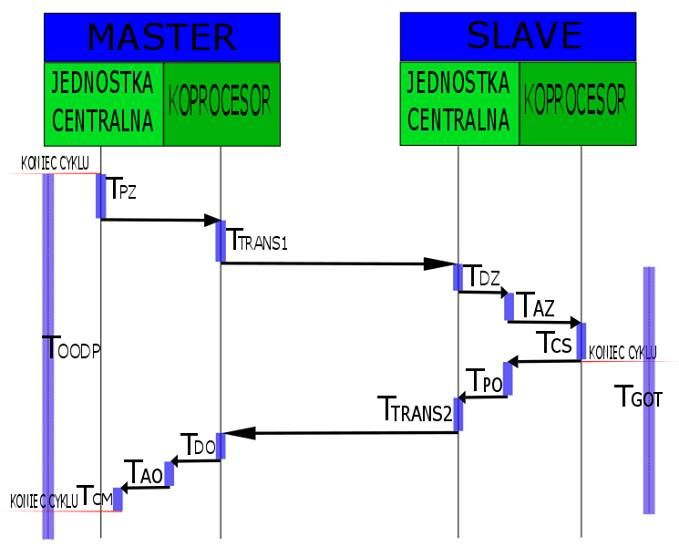
\includegraphics[width=0.7\textwidth]{./img/wymiana.jpg}
		\caption{Przebieg poszczególnych procesów podaczas pojedynczej wymiany}
		\label{fig:wymiana}
	\end{figure}
	\\
	Warto pamiętać, że dla poprawnej pracy sieci powinny zachodzić następujące zależności:
	\begin{equation}
		\label{eq:zalTgot}
		T_{GOT} > T_{DET1} + T_{AZ} + T_{CS} + T_{PO}
	\end{equation}
	\begin{equation}
		\label{eq:zalToodp}
		T_{OODP} > T_{PZ} + T_{TRANS1} + T_{DET1} + T_{AZ} + T_{CS} + T_{PO} + T_{TRANS2} + T_{DO}
	\end{equation}
	Warto zwrócić uwagę na fakt, że w przypadku braku sygnału \textit{końca cyklu $ KC $} w czasie $ T_{GOT} $ koprocesor stacji slave wyśle odpowiedź $ NACK $ powodując uznanie wymiany za nieudaną. Jest to o tyle ważne, że wpływ na to ma czas trwania cyklu automatu slave $ T_{CS} $, którego długości nie da się wyliczyć, a jedynie zmierzyć. Dodatkowo będzie ona się prawdopodobnie zmieniała w zależności od działań podejmowanych przez stację slave, przez co może się drastycznie zmienić w wyniku komunikatów nadanych przez sieć. Takie zdarzenie może zaburzyć działanie sieci - dlatego należy doliczyć pewien margines w stosunku do przewidywanego najdłuższego czasu cyklu.
	\begin{equation}
		\label{eq:czasTrz}
		T_{TR} = \frac{ZT*BT + BS}{P_{TR}}
	\end{equation}
	\begin{equation}
		\label{eq:czasTz}
		T_{TZ} = \frac{ZTZ*BZ + BS}{V}
	\end{equation}
	\begin{equation}
		\label{eq:czasTo}
		T_{TO} = \frac{ZTO*BZ+BS}{V}
	\end{equation}
	\begin{equation}
		\label{eq:czasPW}
		T_{WI} = T_{PZ}+T_{TRANS1} + T_{DZ} + T_{AZ} + T_{CS} + T_{PO} + T_{TRANS2} + T_{DO} + T_{AD} + T_{CM}
	\end{equation}
	\begin{equation}
		\label{eq:czasWW}
		T_{WC} = \sum\limits_{i=1}^N T_{WIi} = \sum\limits_{i=1}^N (T_{PZi} + T_{TRANS1i}) + \sum\limits_{j=1}^N ( + T_{AZj} + T_{CSj} + T_{POj} + T_{TRANS2j}) + \sum\limits_{i=1}^N (T_{CMi}+T_{T_{AOi}} + 2NT_{DO}
	\end{equation}
	\begin{equation}
		\label{eq:czasPO}
		T_{POW} = \sum\limits_{i=1}^N L_{Ri}*T_{TRANS1i} + L_{A}T_{ODDP}
	\end{equation}
	\begin{equation}
		\label{eq:czasMAX}
		T_{WM} = T_{WC} + T_{POW}
	\end{equation}